\documentclass[11pt]{article}
\usepackage[utf8]{inputenc}

\usepackage{amssymb,amsmath}
\usepackage{times,psfrag,epsf,epsfig,graphics,graphicx}
\usepackage{algorithm}
\usepackage{algorithmic}
\usepackage{xcolor}
\usepackage{tikz}

\newcommand\mybox[2][]{\tikz[overlay]\node[fill=blue!20,inner sep=2pt, anchor=text, rectangle, rounded corners=1mm,#1] {#2};\phantom{#2}}


\title{CSCI 338: Quiz ~03~}
\author{William Jardee}
\date{}

\begin{document}

\maketitle

\section*{Problem 1.}

    Based on the reduction from Sorting to 2D Convex Hull that was convered on March 15, suppose that the input for Sorting are given as $x_1 = 4$, $x_2 = -3$, $x_3=1$, $x_4=0$, $x_5 = 3$, $x_6 = -4$, $x_7 = -2$.
    
    \begin{center}
        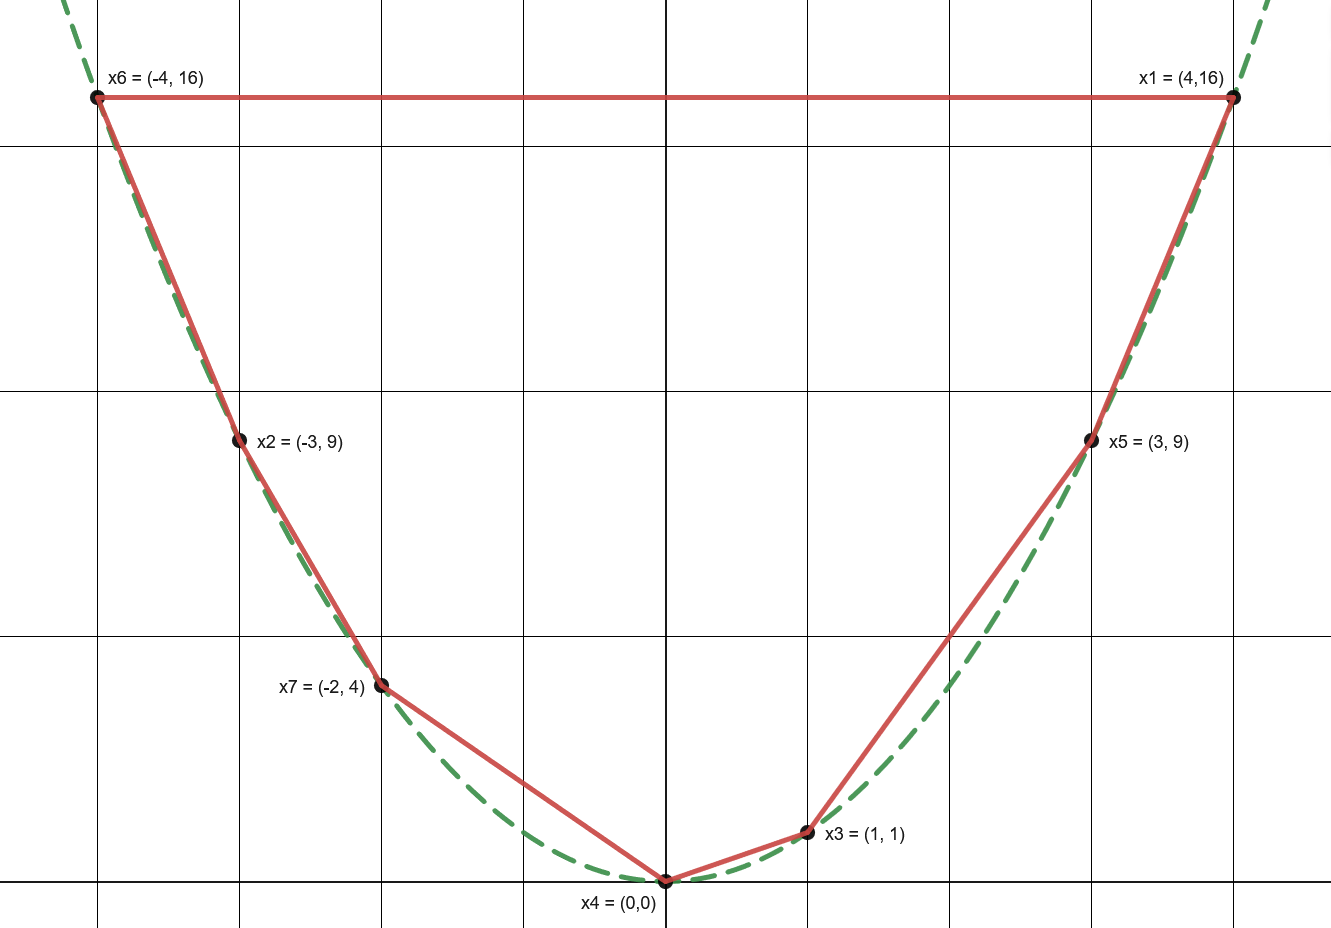
\includegraphics[width = 0.95\linewidth]{images/convexhull.PNG}
    \end{center}
    
    \begin{enumerate}
        \item List the points constructed for the 2D Convex Hull problem. (You must list the coordinates of the points.)\\
        
            Using the $y=x^2$ graph projection: $x_1 = (4, 16)$, $x_2 = (-3, 9)$, $x_3=(1,1)$, $x_4=(0,0)$, $x_5 = (3, 9)$, $x_6 = (-4, 16)$, $x_7 = (-2,4)$
        
        \item Briefly show how the sorted points $x_i$'s are obtained once the 2D convex hull is given.\\
        
            List all the points in the counter-clockwise motion. So, reading off the graph, we get:
            \begin{center}
                $x_6$, $x_2$, $x_7$, $x_4$, $x_3$, $x_5$, $x_1$
            \end{center}
        
        
    \end{enumerate}

\end{document}
